\documentclass{ctexart}
\usepackage[utf8]{inputenc}
\usepackage{geometry}
\usepackage{graphicx}
\usepackage{amsmath}
\usepackage{amssymb}
\usepackage{enumitem}
\usepackage{xcolor}
\usepackage{listings}
\usepackage{threeparttable}
\usepackage{multirow}
\usepackage{longtable}
\geometry{a4paper,left=2cm,right=2cm,top=1.5cm,bottom=1cm}
\newfontfamily\courier{Consolas}
\lstset{linewidth=1.1\textwidth,
		numbers=left, %设置行号位置 
		basicstyle=\small\courier,
		numberstyle=\tiny\courier, %设置行号大小  
		keywordstyle=\color{blue}\courier, %设置关键字颜色  
		%identifierstyle=\bf,
		commentstyle=\it\color[cmyk]{1,0,1,0}\courier, %设置注释颜色 
		stringstyle=\it\color[RGB]{128,0,0}\courier,
		%framexleftmargin=10mm,
		frame=single, %设置边框格式  
		backgroundcolor=\color[RGB]{245,245,244},
		%escapeinside=``, %逃逸字符(1左面的键),用于显示中文  
		breaklines, %自动折行  
		extendedchars=false, %解决代码跨页时,章节标题,页眉等汉字不显示的问题  
		xleftmargin=2em,xrightmargin=2em, aboveskip=1em, %设置边距  
		tabsize=4, %设置tab空格数  
		showspaces=false %不显示空格  
		basicstyle=\small\courier
	   }  
\title{微分方程数值解 - 第十一章上机作业}
\author{樊睿 强基数学 2001 班}
\date{2023年5月27日}

\begin{document}

\maketitle

\begin{abstract}
	本项目实现了八种常微分方程数值解方法:三种多步法(Adam-Bashforth、Adam-Moulton和BDF)、三种龙格库塔方法(Classical RK、ESDIRK和Gauss-Legendre)和两种动态步长龙格库塔方法(Fehlberg 4(5)和Dormand-Prince 5(4)),并将这些方法应用在三星系统中,通过作图和误差分析从实际和理论两个方面分析各方法的效果。

	以下是三种典型的方法对讲义中第一个初值和周期的作图:

	\begin{figure}[htbp]
		\begin{minipage}{5cm}
			\centering
			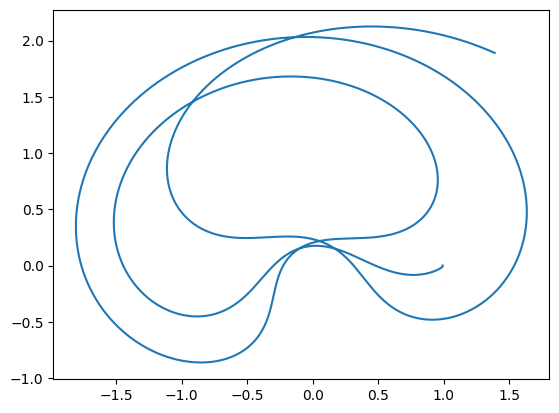
\includegraphics[width = 5cm, height = 4cm]{01.png}
			\caption{Adam-Bashforth, $n=24000$}
			\label{1}
		\end{minipage}
		\begin{minipage}{5cm}
			\centering
			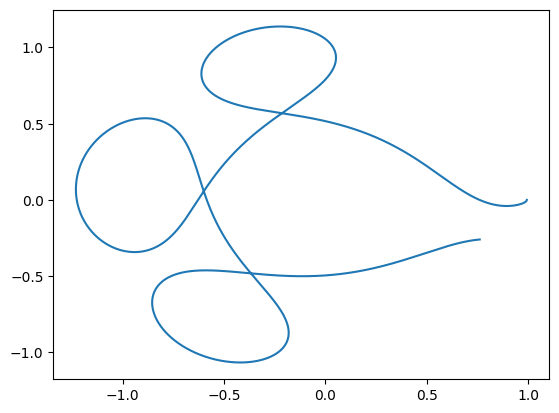
\includegraphics[width = 5cm, height = 4cm]{02.png}
			\caption{Classical-RK, $n=6000$}
			\label{2}
		\end{minipage}
		\begin{minipage}{5cm}
			\centering
			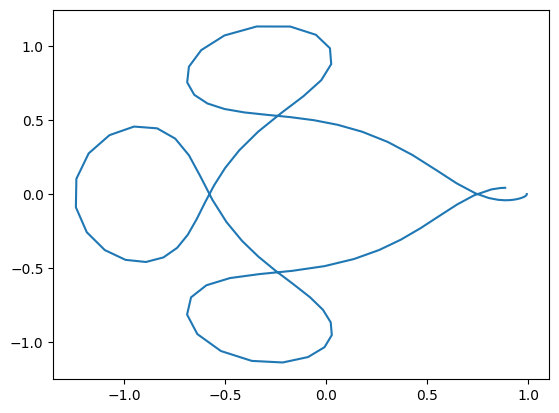
\includegraphics[width = 5cm, height = 4cm]{03.png}
			\caption{Dormand-Prince, 控制步数恰好为 $100$}
			\label{3}
		\end{minipage}
	\end{figure}
\end{abstract}

\section{设计文档}
	IVPSolver类:
	\begin{itemize}
		\item 主要变量和函数:
		\begin{itemize}
			\item Solve函数,输入右端函数$f$、初值$u_0$、终止时间$T$、步数$n$、阶数$s$(该参数仅对多步法有用,其他方法可省略)、是否省略解的细节输出(默认不省略),输出解(vector)。抽象函数。
		\end{itemize}
		\item 继承关系:
		\begin{itemize}
			\item LMM类
			\item RK类
			\item Emb-RK类
		\end{itemize}
	\end{itemize}

	LMM类:
	\begin{itemize}
		\item 主要变量和函数:
		\begin{itemize}
			\item $\alpha$ 数组和 $\beta$ 数组
			\item step函数,输入右端函数$f$、上一步的序号$n$、时间步长$k$、阶数$s$,输出$s$阶多步法的第$n+s$步结果。抽象函数。
		\end{itemize}
		\item 继承关系:
		\begin{itemize}
			\item Adam-Bashforth类
			\item Adam-Moulton类
			\item BDF类
		\end{itemize}
	\end{itemize}
	
	RK类:
	\begin{itemize}
		\item 主要变量和函数:
		\begin{itemize}
			\item 阶数$s$,精度$p$。
			\item $a,b,c$ 数组。
			\item step函数,输入右端函数$f$、上一步的序号$n$、时间步长$k$,输出RK方法的第$n+1$步结果。抽象函数。
		\end{itemize}
		\item 继承关系:
		\begin{itemize}
			\item ERK类,即显式RK方法。ERK类又有子类Classical-4th-RK类。
			\item IRK类,即隐式RK方法。IRK类又有子类ESDIRK类和Gauss类。
		\end{itemize}
	\end{itemize}

	Emb-RK类:
	\begin{itemize}
		\item 主要变量和函数:
		\begin{itemize}
			\item 阶数$s$。
			\item $a,b^0,b^1,c$ 数组。
			\item step函数,输入右端函数$f$、上一步的序号$n$、时间步长$k$,输出Embedded-RK方法的第$n+1$步结果。抽象函数。
		\end{itemize}
	\end{itemize}

	所有IVPSolver类采用对象工厂IVPSolverFactory封装。

\section{多步法的实现和测试}

多步法的实现和单步法非常不同。具体原因在于高阶的多步法需要用到对应的低阶多步法,因此不同阶的多步法不能定义为不同的类,否则无法抽象。

\subsection{多步法求解常微分方程组的实现}

当 $s=1$(即一步法)时,直接令 $U^0=u_0$ 并迭代 $n$ 步即可。

但当 $s>1$ 时,因为我们至少要 $s$ 个初值 $U^0,U^1,\dots,U^{s-1}$,而后 $s-1$ 个初值并非已知,所以我们需要用其他方法计算出这些初值。

最简单的做法是直接用对应的一步法计算。但一步法的误差是 $O(k)$ 的,而我们知道常微分方程组的误差是累乘的,因此这会导致最终用高阶多步法解出的答案和用一步法解出的答案差不多。这样高阶多步法就失去意义了。

另一种做法是用高阶单步法(例如四阶RK方法、三阶Gauss-Legerand方法等)计算前 $s-1$ 个初值,这样可以保证高阶多步法的精度。但这样在使用多步法的同时还要使用其他单步法,某种意义上也使多步法失去了它的精髓。

本项目中采取的做法是使用 $s-1$ 阶单步法计算前 $s-1$ 个初值,但缩短时间步长。设原 $s$ 阶多步法步长为 $k$,则令 $s-1$ 阶单步法步长为 $k^{\frac s{s-1}}$。

当然,如果 $s-1\geq 2$,这 $s-1$ 个初值也不能直接计算。因此要继续递归,直到 $s=1$ 为止。

然而,这样又引出了下一个问题。例如我们取 $T=1,s=4,k=10^{-4}$,则递归到 $s=1$ 时,我们需要以 $10^{-16}$ 的步长计算 $t=10^{-8}$ 处的值。这样需要迭代 $10^8$ 步!这远远超过了原本所需迭代的次数 $10^4$。

不难证明只有 $s=2$ 时下一步递归会出现这种情况。考虑倍增优化,设 $s=2$ 时步长为 $k$,我们先用单步法计算 $0,k^2$ 处的值,然后用 $s=2$ 的多步法以 $0,k^2$ 处的初值计算 $2k^2$ 处的值,再用 $0,2k^2$ 处的初值计算 $4k^2$ 处的值,直到计算出 $k$ 处的值为止。

这样第一步的误差是 $O(k^2)$,而后面每一步的误差都至多 $O(k^2)$。步数是 $O(\log k)$。这样就避免了严重耗时的问题。

三种多步法的求解函数没有本质区别,因此直接定义在父类中了。

\begin{lstlisting}[language=c++][htbp]
class LMM : public IVPSolver{
	protected:
		virtual void step(const Function_nd<double>& f, int n, double k, int s) = 0;
	public:
		virtual vector<Colvec<double>> Solve(const Function_nd<double>& f, const Colvec<double>& u0, double T, int n, int s = 0, bool omit = 0) {
			long long start = chrono::steady_clock::now().time_since_epoch().count();
			double k = T/n;
			u.resize(1);
			u[0] = u0;
			if (s>1) {
				if (s>2) {
					double _k = pow(k, 1.0*s/(s-1));
					int m = k / _k;
					vector<Colvec<double>> v = Solve(f, u0, k*(s-1), m*(s-1), s-1, 1);
					u.resize(s);
					for (int i = 1; i <= s-1; ++ i) u[i] = v[i*m];
				}
				else {
					double m = 1;
					while (m < 1/k) m *= 2;
					double kk = k/m;
					u.resize(3);
					step(f, 0, kk, 1);
					for (double i = 1; i < m; i *= 2) {
						step(f, 0, kk*i, 2);
						u[1] = u[2];
					}
				}
			}
			u.resize(n+1);
			for (int i = s; i <= n; ++ i) step(f, i-s, k, s);
			long long end = chrono::steady_clock::now().time_since_epoch().count();
			if (!omit) {
				cout << "============LMM Method Return============" << endl;
				cout << "Method: " << method_name << endl;
				cout << "Stage: " << s << endl;
				cout << "Start time: 0, Terminal time: " << T << endl;
				cout << "Steps: " << n << endl;
				cout << "CPU Time: " << (end - start) * 1e-6 << endl;
				cout << "Error: " << ~(u[n] - u[0]) << endl;
				cout << "2-norm of Error: " << vert_2(u[n] - u[0]) << endl;
				cout << "=========================================" << endl;
			}
			return u;
		}
	};
\end{lstlisting}

\subsection{多步法一步迭代的实现}

因为三种多步法的迭代格式有很大不同,所以我们没有必要将它们的step函数统一实现:这反而会带来不必要的时间消耗。

\subsubsection{Adam-Bashforth方法一步迭代的实现}

Adam-Bashforth方法是显式多步法,可以直接计算。因为只有 $\alpha_s=1$,所以我们无需定义 $\alpha$ 数组,只需定义 $\beta$ 数组即可。

\begin{lstlisting}[language=c++]
class Adam_Bashforth : public LMM {
protected:
	vector<double> beta[5];
	virtual void step(const Function_nd<double>& f, int n, double k, int s) {
		u[n+s] = u[n+s-1];
		for (int i = 0; i <= s-1; ++ i)
			u[n+s] += k * beta[s][i] * f(u[n+i]);
	}
public:
	Adam_Bashforth()  {
		method_name = "Adam-Bashforth";
		beta[1] = {1};
		beta[2] = {-1/2.0, 3/2.0};
		beta[3] = {5/12.0, -16/12.0, 23/12.0};
		beta[4] = {-9/24.0, 37/24.0, -59/24.0, 55/24.0};
	}
};
\end{lstlisting}

\subsubsection{Adam-Moulton方法和BDF方法一步迭代的实现}

Adam-Moulton方法和BDF方法都是隐式多步法,需要迭代计算。即:先假设 $U^{n+1}=U^n$,代入计算公式的右端项,然后比较计算结果和 $U^{n+1}$ 的大小,若小于某个定值 $\epsilon$(本项目中定为 $10^{-14}$),则接受当前结果,否则继续迭代。

同样的,Adam-Moulton方法只需定义 $\beta$ 数组,BDF方法只需定义 $\alpha$ 数组和 $\beta_s$ 的值。

\begin{lstlisting}[language=c++]
class Adam_Moulton : public LMM {
	protected:
		vector<double> beta[5];
		virtual void step(const Function_nd<double>& f, int n, double k, int s) {
			u[n+s] = u[n+s-1];
			Colvec<double> last, now;
			do {
				now = u[n+s-1];
				for (int i = 0; i <= s; ++ i)
					now += k * beta[s][i] * f(u[n+i]);
				last = u[n+s];
				u[n+s] = now;
			} while (vert_2(last - now) > 1e-14);
		}
	public:
		Adam_Moulton() {
			method_name = "Adam-Moulton";
			beta[1] = {1/2.0, 1/2.0};
			beta[2] = {-1/12.0, 8/12.0, -5/12.0};
			beta[3] = {1/24.0, -5/24.0, 19/24.0, 9/24.0};
			beta[4] = {-19/720.0, 106/720.0, -264/720.0, 646/720.0, 251/720.0};
		}
	};
	
	class BDF : public LMM {
	protected:
		vector<double> alpha[5];
		double beta[5];
		virtual void step(const Function_nd<double>& f, int n, double k, int s) {
			u[n+s] = u[n+s-1];
			Colvec<double> last, now;
			do {
				now = k * beta[s] * f(u[n+s]);
				for (int i = 0; i <= s-1; ++ i)
					now -= alpha[s][i] * u[n+i];
				last = u[n+s];
				u[n+s] = now;
			} while (vert_2(last - now) > 1e-14);
		}
	public:
		BDF() {
			method_name = "BDF";
			beta[1] = 1,		alpha[1] = {-1};
			beta[2] = 2/3.0,	alpha[2] = {1/3.0, -4/3.0};
			beta[3] = 6/11.0,	alpha[3] = {-2/11.0, 9/11.0, -18/11.0};
			beta[4] = 12/25.0,	alpha[4] = {3/25.0, -16/25.0, 36/25.0, -48/25.0};
		}
	};
\end{lstlisting}

\subsection{多步法的求解结果和误差分析}

对课件中给出的(修改后的)第一个初始条件,分别运行三种多步法 $s=1,2,3,4$ 的版本,误差用二范数,时间单位毫秒,作表格。

\begin{table}\centering
	\resizebox{0.75\columnwidth}{!}{
	\begin{tabular}{|c|c|c|c|c|c|c|c|c|c|c|c|c|}
	\hline
	\multirow{2}{*}{迭代步数} & \multicolumn{3}{c|}{$s=1$} & \multicolumn{3}{c|}{$s=2$} & \multicolumn{3}{c|}{$s=3$} & \multicolumn{3}{c|}{$s=4$} \\ \cline{2-13}
	& 误差 & 时间 & 收敛阶 & 误差 & 时间 & 收敛阶 & 误差 & 时间 & 收敛阶 & 误差 & 时间 & 收敛阶\\ \cline{1-13}
	$5\times 10^5$ & 1.79e+00 & 647  & - & 8.38e-01 & 1278 & - & 3.96e-03 & 1936 & - & 4.57e-04 & 2537 & - \\ \cline{1-13}
	$1\times 10^6$ & 1.71e+00 & 1426 & 0.07 & 2.00e-01 & 2597 & 2.07 & 5.17e-04 & 3862 & 2.93 & 2.89e-05 & 4925 & 3.98\\ \cline{1-13}
	$2\times 10^6$ & 1.59e+00 & 2837 & 0.10 & 4.84e-02 & 5126 & 2.05 & 6.60e-05 & 7730 & 2.97 & 1.82e-06 & 9703 & 4.16\\ \cline{1-13}
	\end{tabular}}
	\caption{Adam-Bashforth方法的误差和效率}
\end{table}

\begin{table}\centering
	\resizebox{0.75\columnwidth}{!}{
	\begin{tabular}{|c|c|c|c|c|c|c|c|c|c|c|c|c|}
	\hline
	\multirow{2}{*}{迭代步数} & \multicolumn{3}{c|}{$s=1$} & \multicolumn{3}{c|}{$s=2$} & \multicolumn{3}{c|}{$s=3$} & \multicolumn{3}{c|}{$s=4$} \\ \cline{2-13}
	& 误差 & 时间 & 收敛阶 & 误差 & 时间 & 收敛阶 & 误差 & 时间 & 收敛阶 & 误差 & 时间 & 收敛阶\\ \cline{1-13}
	$5\times 10^5$ & 1.46e-01 & 5848 & - & 3.11e+00 & 7746 & - & 1.83e-01 & 9526 & - & 4.44e-03 & 11239 & - \\ \cline{1-13}
	$1\times 10^6$ & 3.79e-02 & 10757 & 1.95 & 3.08e+00 & 13850 & - & 5.21e-02 & 18293 & 1.81 & 9.86e-04 & 22053 & 2.17 \\ \cline{1-13}
	$2\times 10^6$ & 9.55e-03 & 19692 & 1.99 & 3.07e+00 & 27927 & - & 1.53e-02 & 35342 & 1.77 & 2.40e-04 & 45365 & 2.03 \\ \cline{1-13}
	\end{tabular}}
	\caption{Adam-Moulton方法的误差和效率}
\end{table}

\begin{table}\centering
	\resizebox{0.75\columnwidth}{!}{
	\begin{tabular}{|c|c|c|c|c|c|c|c|c|c|c|c|c|}
	\hline
	\multirow{2}{*}{迭代步数} & \multicolumn{3}{c|}{$s=1$} & \multicolumn{3}{c|}{$s=2$} & \multicolumn{3}{c|}{$s=3$} & \multicolumn{3}{c|}{$s=4$} \\ \cline{2-13}
	& 误差 & 时间 & 收敛阶 & 误差 & 时间 & 收敛阶 & 误差 & 时间 & 收敛阶 & 误差 & 时间 & 收敛阶\\ \cline{1-13}
	$5\times 10^5$ & 2.10e+00 & 5981 & - & 4.96e-01 & 5812 & - & 2.53e-03 & 6748 & - & 2.62e-04 & 6958 & - \\ \cline{1-9}
	$1\times 10^6$ & 2.12e+00 & 8040 & - & 1.46e-01 & 9457 & 1.76 & 3.36e-04 & 11283 & 2.91 & 1.73e-05 & 12726 & 3.92 \\ \cline{1-9}
	$2\times 10^6$ & 2.33e+00 & 14604 & - & 3.78e-02 & 17695 & 1.94 & 4.09e-05 & 20293 & 3.03 & 2.40e-06 & 23632 & 2.85\\ \cline{1-9}
	\end{tabular}}
	\caption{BDF方法的误差和效率}
\end{table}

从这几张表中可以看出:
\begin{enumerate}
	\item $s=2,3,4$ 的 Adam-Bashforth 方法、$s=1$ 的 Adam-Moulton 方法和 $s=2,3,4$ 的 BDF 方法均正常收敛且收敛阶正确。
	\item $s=1$ 的 Adam-Bashforth 方法要收敛需要的算力太大,至少在 $n$ 取 $2\times 10^6$ 时还没有较稳定地收敛。
	\item $s=2$ 的 Adam-Moulton 方法和 $s=1$ 的 BDF 方法可能在迭代过程中超出了不动点迭代的收敛域,导致最终没有收敛。
	\item $s=3,4$ 的 Adam-Moulton 方法虽然阶数很高且迭代过程没有发散,但因为它们前 $s-1$ 步用到了不收敛的 $s=2$ 方法,导致也只能体现出二阶的收敛性。
	\item 从程序的输出(不是表格的输出)可以发现,$u_1$ 和 $u_2$ 的误差明显小于 $u_4$ 和 $u_5$。
	\item 隐式方法耗时一般明显高于同阶显式方法。
\end{enumerate}

下面分别给出三种方法的最高阶方法对第一组初值和周期的作图。两个周期。

\begin{figure}[htbp]
	\begin{minipage}{5cm}
		\centering
		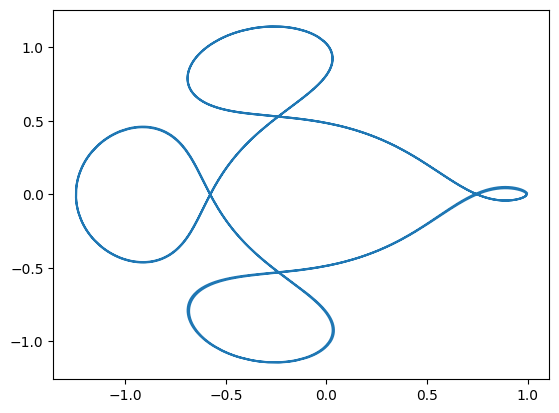
\includegraphics[width = 5cm, height = 4cm]{11.png}
		\caption{Adam-Bashforth, $s=4,n=500000$}
		\label{11}
	\end{minipage}
	\begin{minipage}{5cm}
		\centering
		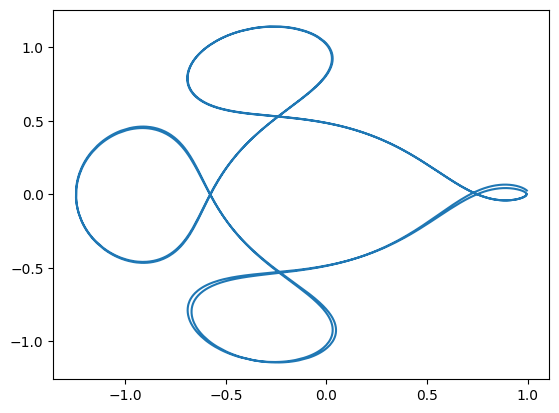
\includegraphics[width = 5cm, height = 4cm]{12.png}
		\caption{Adam-Moulton, $s=4,n=500000$}
		\label{12}
	\end{minipage}
	\begin{minipage}{5cm}
		\centering
		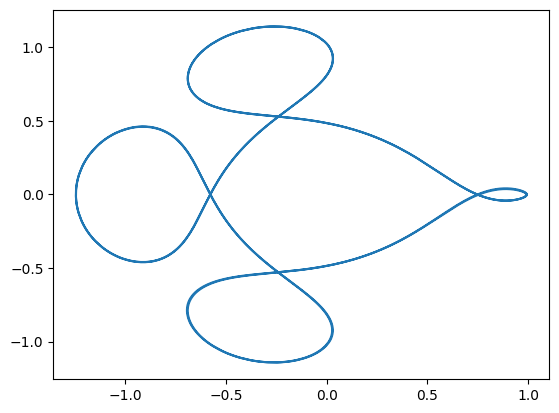
\includegraphics[width = 5cm, height = 4cm]{13.png}
		\caption{BDF, $s=4,n=500000$}
		\label{13}
	\end{minipage}
\end{figure}

Adam-Bashforth方法和BDF方法在两个周期时基本稳定,但Adam-Moulton方法已发生明显偏移。

\section{龙格库塔方法的实现和测试}

\subsection{龙格库塔方法求解常微分方程组以及外插法误差估计的实现}

龙格库塔方法是单步法,所以只需和 $s=1$ 的多步法一样实现即可。

外插法误差估计是用单步迭代结果和用一半步长做两步迭代的结果作比较,再乘 $\dfrac {2^p}{1-2^p}$ 估计出结果。

\begin{lstlisting}[language=c++]
class RK : public IVPSolver{
	protected:
		int s, p;
		vector<vector<double>> a;
		vector<double> b, c;
		virtual Colvec<double> step(const Function_nd<double>& f, const Colvec<double>& u, double k) = 0;
	public:
		virtual vector<Colvec<double>> Solve(const Function_nd<double>& f, const Colvec<double>& u0, double T, int n, int s = 0, bool omit = 0) {
			long long start = chrono::steady_clock::now().time_since_epoch().count();
			double k = T/n;
			u.resize(n+1);
			u[0] = u0;
			for (int i = 0; i < n; ++ i) u[i+1] = step(f, u[i], k);
			long long end = chrono::steady_clock::now().time_since_epoch().count();
			if (!omit) {
				cout << "============RK Method Return============" << endl;
				cout << "Method: " << method_name << endl;
				cout << "Stages: " << s << endl;
				cout << "Start time: 0, Terminal time: " << T << endl;
				cout << "Steps: " << n << endl;
				cout << "CPU Time: " << (end - start) * 1e-6 << endl;
				cout << "Error: " << ~(u[n] - u[0]) << endl;
				Colvec<double> u_half, err(f.n);
				for (int i = 0; i < n; ++ i) {
					u_half = step(f, step(f, u[i], k/2), k/2);
					for (int j = 0; j < f.n; ++ j) err[j] += fabs(u[i+1][j] - u_half[j]) * (1<<p) / ((1<<p)-1);
				}
				cout << "Error Estimated by Richardson extrapolation: " << ~err << endl;
				cout << "=================================================" << endl;
			}
			return u;
		}
	};	
\end{lstlisting}

\subsection{龙格库塔方法一步迭代的实现}

所有龙格库塔方法的迭代格式相差都不多。如根据方法特性(对角、显式对角等)单独设计每种方法的迭代,耗时费力且作用不大。因此这里对所有龙格库塔方法进一步分类,仅分为显示龙格库塔方法(ERK)和隐式龙格库塔方法(IRK)。

\subsubsection{ERK方法一步迭代的实现}

ERK方法类似显式多步法,直接根据公式计算即可依次得到每个stage的结果。

\begin{lstlisting}[language=c++]
class ERK : public RK {
	protected:
		virtual Colvec<double> step(const Function_nd<double>& f, const Colvec<double>& u, double k) {
			vector<Colvec<double>> y(s);
			for (int i = 0; i < s; ++ i) {
				Colvec<double> r = u;
				for (int j = 0; j < i; ++ j)
					r += k * a[i][j] * y[j];
				y[i] = f(r);
			}
			Colvec<double> res = u;
			for (int i = 0; i < s; ++ i) 
				res += k * b[i] * y[i];
			return res;
		}
	};
\end{lstlisting}

它的子类即经典四阶RK方法。

\begin{lstlisting}
class Classical_4th_RK : public ERK {
	public:
		Classical_4th_RK() {
			method_name = "Classical RK";
			s = 4, p = 4;
			a = {
				{0, 0, 0, 0},
				{0.5, 0, 0, 0},
				{0, 0.5, 0, 0},
				{0, 0, 1, 0}
			};
			b = {1/6.0, 1/3.0, 1/3.0, 1/6.0};
			c = {0, 0.5, 0.5, 1};
		}
	};
\end{lstlisting}

\subsubsection{IRK方法一步迭代的实现}

IRK方法类似隐式多步法,初始令所有的 $U^{n+1}=U^n,y_i = f(U^n)$,代入迭代公式右端计算出 $U^{n+1}$。若计算结果与上次迭代结果差不超过 $\epsilon=10^{-14}$,则接受结果;否则继续迭代。

\begin{lstlisting}
class IRK : public RK {
	protected:
		virtual Colvec<double> step(const Function_nd<double>& f, const Colvec<double>& u, double k) {
			vector<Colvec<double>> y(s);
			for (int i = 0; i < s; ++ i) y[i] = f(u);
			Colvec<double> res = u;
			Colvec<double> last, now;
			do {
				vector<Colvec<double>> ny(s);
				for (int i = 0; i < s; ++ i) {
					Colvec<double> r = u;
					for (int j = 0; j < s; ++ j)
						r += k * a[i][j] * y[j];
					ny[i] = f(r);
				}
				now = u;
				for (int i = 0; i < s; ++ i)
					now += k * b[i] * ny[i];
				last = res;
				res = now;
				y = ny;
			} while(vert_2(last - now) > 1e-14);
			return res;
		}
	};
\end{lstlisting}

它的子类即ESDIRK方法和高斯勒让德方法。

\begin{lstlisting}[language=c++]
class ESDIRK : public IRK {
public:
	ESDIRK() {
		method_name = "ESDIRK";
		s = 6, p = 4;
		a = {
			{0, 0, 0, 0, 0, 0},
			{1/4.0, 1/4.0, 0, 0, 0, 0},
			{8611/62500.0, -1743/31250.0, 1/4.0, 0, 0, 0},
			{5012029.0/34652500.0, -654441.0/2922500.0, 174375.0/388108.0, 1/4.0, 0, 0},
			{15267082809.0/155376265600.0, -71443401.0/120774400.0, 730878875.0/902184768.0, 2285395.0/8070912.0, 1/4.0, 0},
			{82889/524892.0, 0, 15625/83664.0, 69875/102672.0, -2260/8211.0, 1/4.0}
		};
		b = a[5];
		c = {0, 1/2.0, 83/250.0, 31/50.0, 17/20.0, 1};
	}
};

class Gauss : public IRK {
public:
	Gauss(int s) {
		method_name = "Gauss-Legendre";
		RK::s = s, p = 2*s;
		if (s == 1) {
			a = {{0.5}};
			b = {1};
			c = {0.5};
		}
		else if (s == 2) {
			double q = sqrt(3);
			a = {
				{1.0/4, (3-2*q)/12},
				{(3+2*q)/12, 1.0/4}
			};
			b = {0.5, 0.5};
			c = {(3-q)/6, (3+q)/6};
		}
		else if (s == 3) {
			double q = sqrt(15);
			a = {
				{5.0/36, 2.0/9-q/15, 5.0/36-q/30},
				{5.0/36+q/24, 2.0/9, 5.0/36-q/24},
				{5.0/36+q/30, 2.0/9+q/15, 5.0/36}
			};
			b = {5.0/18, 4.0/9, 5.0/18};
			c = {(5-q)/10, 1.0/2, (5+q)/10};
		}
	}
};
\end{lstlisting}

\subsection{RK方法的求解结果和误差分析}

对课件中给出的(修改后的)第一个初始条件,分别运行三种RK方法,误差用二范数,时间单位毫秒,作表格。

\begin{table}\centering
	\resizebox{0.75\columnwidth}{!}{
	\begin{tabular}{|c|c|c|c|c|c|c|c|c|c|c|c|c|c|c|c|c|}
	\hline
	\multirow{2}{*}{迭代步数} & \multicolumn{3}{c|}{经典RK} & \multicolumn{3}{c|}{ESDIRK} & \multicolumn{3}{c|}{Gauss,$s=1$} & \multicolumn{3}{c|}{Gauss,$s=2$} & \multicolumn{3}{c|}{Gauss,$s=3$}\\ \cline{2-16}
	& 误差 & 时间 & 收敛阶 & 误差 & 时间 & 收敛阶 & 误差 & 时间 & 收敛阶 & 误差 & 时间 & 收敛阶 & 误差 & 时间 & 收敛阶\\ \cline{1-16}
	$5\times 10^4$ & 9.45e-03 & 458 & - & 3.19e-03 & 5010 & - & 2.11e+00 & 562 & - & 2.13e-03 & 1103 & - & 1.69e-06 & 1853 & - \\ \cline{1-16}
	$1\times 10^5$ & 5.57e-04 & 874 & 4.08 & 2.00e-04 & 9512 & 3.99 & - & - & - & 1.34e-04 & 2071 & 3.99 & 2.63e-08 & 3452 & 6.01\\ \cline{1-16}
	$2\times 10^5$ & 3.37e-05 & 1785 & 4.04 & 1.25e-05 & 19078 & 4.00 & 1.11e+00 & 2130 & 0.47 & 8.38e-06 & 4197 & 3.99 & 1.07e-09 & 7022 & 4.61 \\ \cline{1-16}
	$4\times 10^5$ & 2.08e-06 & 3503 & 4.01 & 7.86e-07 & 36349 & 3.99 & 2.70e-01 & 4337 & 2.04 & 5.23e-07 & 8272 & 4.00 & 3.45e-10 & 13431 & 1.63\\ \cline{1-16}
	\end{tabular}}
	\caption{各种RK方法的误差和效率}
\end{table}

从这张表中可以看出:
\begin{enumerate}
	\item 同阶下,单步法明显比多步法稳定且精确。上面三种四阶单步法(经典四阶RK、ESDIRK、二阶Gauss-Legendre)在 $n=4\times 10^5$ 时的误差都明显小于任何多步法在 $n=2\times 10^6$ 时的误差。
	\item 虽然精度阶数相同,但从常数上,经典四阶RK方法、ESDIRK方法、二阶高斯方法的精度从低到高。
	\item 一阶Gauss方法精度太低,在 $n$ 较小时很不稳定,甚至不收敛(短横线意为不收敛)。
	\item 三阶Gauss方法在 $n=5\times 10^4$ 时收敛阶已经稳定,但在 $n=2\times 10^5$ 时收敛阶又发生了变化。这是因为它的主要误差来源已经是机器精度了。
	\item 经典RK方法的耗时最短,因为它是显式方法。高斯方法次之,ESDIRK方法最慢。
\end{enumerate}

我们再对第二个初始条件和周期使用外插法估计误差,并与实际误差比较。

\begin{table}\centering
	\resizebox{0.75\columnwidth}{!}{
	\begin{tabular}{|c|c|c|c|c|c|c|c|c|c|c|c|c|c|c|c|}
	\hline
	\multirow{2}{*}{迭代步数} & \multicolumn{3}{c|}{经典RK} & \multicolumn{3}{c|}{ESDIRK} & \multicolumn{3}{c|}{Gauss,$s=1$} & \multicolumn{3}{c|}{Gauss,$s=2$} & \multicolumn{3}{c|}{Gauss,$s=3$}\\ \cline{2-16}
	& 误差 & 外插法误差 & 收敛阶 & 误差 & 外插法误差 & 收敛阶 & 误差 & 外插法误差 & 收敛阶 & 误差 & 外插法误差 & 收敛阶 & 误差 & 外插法误差 & 收敛阶\\ \cline{1-16}
	$5\times 10^3$ & 2.98e-07 & 7.65e-08 & - & 8.51e-08 & 1.19e-07 & - & 5.93e-03 & 4.34e-03 & - & 2.25e-07 & 1.38e-07 & - & 7.50e-11 & 3.64e-12 & - \\ \cline{1-16}
	$1\times 10^4$ & 5.70e-09 & 4.78e-09 & 4.00 & 3.82e-09 & 7.45e-09 & 4.00 & 1.49e-03 & 1.08e-03 & 2.01 & 1.40e-08 & 8.62e-09 & 4.00 & 8.35e-11 & 8.70e-13 & 2.06\\ \cline{1-16}
	$2\times 10^4$ & 6.57e-10 & 2.99e-10 & 4.00 & 1.13e-10 & 4.66e-10 & 3.50 & 3.70e-04 & 2.71e-04 & 1.99 & 7.95e-10 & 5.39e-10 & 4.00 & 8.30e-11 & 1.73e-12 & - \\ \cline{1-16}
	\end{tabular}}
	\caption{各种RK方法的误差和外插法误差}
\end{table}

可见外插法的误差估计在数量级上是准确的,且也基本反映了各方法的收敛阶。但当误差主要来源为机器精度时,它估计的收敛阶同样会出错。

下面分别给出三种方法(高斯勒让德方法取 $s=3$)对第一组初值和周期的作图。三个周期。

\begin{figure}[htbp]
	\begin{minipage}{5cm}
		\centering
		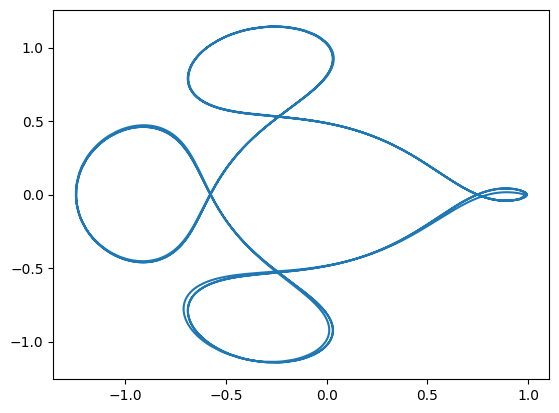
\includegraphics[width = 5cm, height = 4cm]{21.png}
		\caption{Classical RK, $n=500000$}
		\label{21}
	\end{minipage}
	\begin{minipage}{5cm}
		\centering
		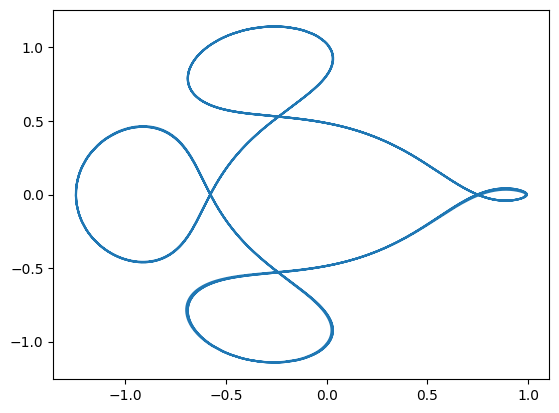
\includegraphics[width = 5cm, height = 4cm]{22.png}
		\caption{ESDIRK, $n=500000$}
		\label{22}
	\end{minipage}
	\begin{minipage}{5cm}
		\centering
		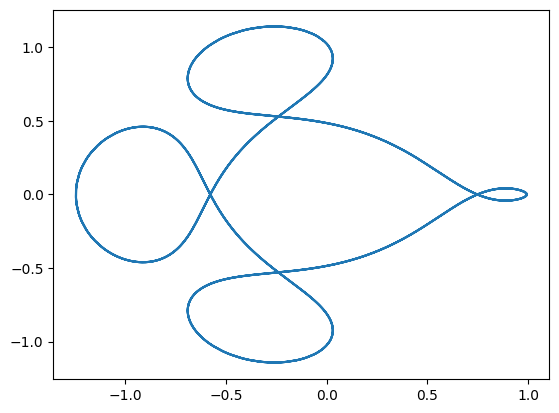
\includegraphics[width = 5cm, height = 4cm]{23.png}
		\caption{Gauss-Legendre, $s=3,n=500000$}
		\label{23}
	\end{minipage}
\end{figure}

Classical RK 方法出现了明显的偏移,ESDIRK 方法也略有偏移。Gauss-Legendre方法仍较稳定。

\section{可变步长龙格库塔方法的实现和测试}

\subsection{可变步长龙格库塔方法的实现}

本项目实现的两个可变步长方法都是显式方法。因此可统一实现。

可变步长龙格库塔方法是两个 $a,c$ 相同、精度分别为 $p$ 阶和 $\hat{p}$ 阶的方法嵌套在一起,故又称为嵌套龙格库塔方法。它通过两个方法算出的解的误差来控制步长,使求解器在需要精密计算的时间段缩短步长,可以粗放计算的时间段增大步长。

一步迭代的主要步骤如下:

\begin{enumerate}
	\item 用两种RK方法分别计算一步迭代的结果 $U^{n+1},\hat{U}^{n+1}$。
	\item 令 $E_{ind}=\sqrt{\frac 1N\sum_{i=1}^N(\frac {U^{n+1}-\hat{U}^{n+1}}{\epsilon_i})^2}$,$\epsilon_i = \epsilon(1+|U^n_i|)$。
	\item 令 $k\leftarrow k\min\{\rho_{\max},\max\{\rho_{min},\rho(E_{ind})^{\frac {-1}{q+1}}\}\}$,其中 $q=\min\{p,\hat{p}\},\rho_{\max}=5,\rho=0.8,\rho_{\min}=0.2$。
	\item 若 $E_{ind}\leq 1$,则进行下一步迭代;否则重新进行这步迭代。
\end{enumerate}

\begin{lstlisting}[language=c++]
class Emb_RK : public IVPSolver{
	#define err_tolerance 1e-14
	#define rho_max 5.0
	#define rho_min 0.2
	#define rho 0.8
	#define k_max 1.0
protected:
	int s, p[2];
	vector<vector<double>> a;
	vector<double> b[2], c;
	vector<double> t;
	Colvec<double> step(const Function_nd<double>& f, const Colvec<double>& u, double k, bool o) {
		vector<Colvec<double>> y(s);
		for (int i = 0; i < s; ++ i) {
			Colvec<double> r = u;
			for (int j = 0; j < i; ++ j)
				r += k * a[i][j] * y[j];
			y[i] = f(r);
		}
		Colvec<double> res = u;
		for (int i = 0; i < s; ++ i) 
			res += k * b[o][i] * y[i];
		return res;
	}
	double E_ind(const Colvec<double>& u, const Colvec<double>& e) {
		double res = 0;
		for (int i = 0; i < e.row(); ++ i)
			res += pow(fabs(e[i]) / (err_tolerance * (1 + fabs(u[i]))), 2);
		return sqrt(res / e.row());
	}
public:
	virtual vector<Colvec<double>> Solve(const Function_nd<double>& f, const Colvec<double>& u0, double T, int n = 10000, int s = 0, bool omit = 0) {
		long long start = chrono::steady_clock::now().time_since_epoch().count();
		double k = T/n;
		u.push_back(u0);
		t.push_back(0);
		n = 0;
		while (t[n] < T) {
			if (t[n] + k > T) k = T - t[n];
			Colvec<double> u0, u1;
			double e;
			do{
				u0 = step(f, u[n], k, 0);
				u1 = step(f, u[n], k, 1);
				e = E_ind(u[n], u0-u1);
				k *= min(rho_max, max(rho_min, rho * pow(e, -1.0/(min(p[0], p[1])+1))));
				k = min(k, k_max);
			}while(e > 1);
			u.push_back(u0);
			t.push_back(t[n] + k);
			++n;
		}
		long long end = chrono::steady_clock::now().time_since_epoch().count();
		if (!omit) {
			cout << "============Embedded RK Method Return============" << endl;
			cout << "Method: " << method_name << endl;
			cout << "Stage: " << s << endl;
			cout << "Start time: 0, Terminal time: " << T << endl;
			cout << "Steps: " << n << endl;
			cout << "CPU Time: " << (end - start) * 1e-6 << endl;
			cout << "Error: " << ~(u[n] - u[0]) << endl;
			cout << "2-norm of Error: " << vert_2(u[n] - u[0]) << endl;
			cout << "========================================" << endl;
		}
		return u;
	}
};
\end{lstlisting}

两个子类 Fehlberg-Emb-RK 和 Dormand-Prince-Emb-RK:

\begin{lstlisting}[language=c++]
class Fehlberg_Emb_RK : public Emb_RK {
public:
	Fehlberg_Emb_RK() {
		method_name = "Fehlberg 4(5) embedded RK";
		s = 6, p[0] = 4, p[1] = 5;
		a = {
			{0, 0, 0, 0, 0, 0},
			{1.0/4, 0, 0, 0, 0, 0},
			{3.0/32, 9.0/32, 0, 0, 0, 0},
			{1932.0/2197, -7200.0/2197, 7296.0/2197, 0, 0, 0},
			{439.0/216, -8, 3680.0/513, -845.0/4104, 0, 0},
			{-8.0/27, 2, -3544.0/2565, 1859.0/4104, -11.0/40, 0},
		};
		b[0] = {25.0/216, 0, 1408.0/2565, 2197.0/4104, -1.0/5, 0};
		b[1] = {16.0/135, 0, 6656.0/12825, 28561.0/56430, -9.0/50, 2.0/55};
		c = {0, 1.0/4, 3.0/8, 12.0/13, 1, 1.0/2};
	}
};

class Dormand_Prince_Emb_RK : public Emb_RK {
public:
	Dormand_Prince_Emb_RK() {
		method_name = "Dormand-Prince 5(4) embedded RK";
		s = 7, p[0] = 5, p[1] = 4;
		a = {
			{0, 0, 0, 0, 0, 0, 0},
			{1.0/5, 0, 0, 0, 0, 0, 0},
			{3.0/40, 9.0/40, 0, 0, 0, 0, 0},
			{44.0/45, -56.0/15, 32.0/9, 0, 0, 0, 0},
			{19372.0/6561, -25360.0/2187, 64448.0/6561, -212.0/729, 0, 0, 0},
			{9017.0/3168, -355.0/33, 46732.0/5247, 49.0/176, -5103.0/18656, 0, 0},
			{35.0/384, 0, 500.0/1113, 125.0/192, -2187.0/6784, 11.0/84, 0}
		};
		b[0] = a[6];
		b[1] = {5179.0/57600, 0, 7571.0/16695, 393.0/640, -92097.0/339200, 187.0/2100, 1.0/40};
		c = {0, 1.0/5, 3.0/10, 4.0/5, 8.0/9, 1, 1};
	}
};
\end{lstlisting}

\subsection{可变长龙格库塔方法的求解结果和误差分析}

对课件中给出的(修改后的)第一个初始条件,分别运行两种RK方法,初始步长为 $\dfrac T{10^6}$,得出如下结果(误差用二范数,时间单位毫秒)。

\begin{table}\centering
	\resizebox{0.75\columnwidth}{!}{
	\begin{tabular}{|c|c|c|c|c|c|}
	\hline
	\multicolumn{3}{|c|}{Fehlberg} & \multicolumn{3}{c|}{Dormand-Prince} \\ \cline{1-6}
	误差 & 步数 & 时间 & 误差 & 步数 & 时间 \\ \cline{1-6}
	8.53e-06 & 5896 & 196 & 8.63e-06 & 5420 & 231 \\ \cline{1-6}
	\end{tabular}}
	\caption{可变长龙格库塔方法的误差、步数和效率}
\end{table}

由上表可知:
\begin{enumerate}
	\item 可变长龙格库塔方法相比同阶的RK方法如经典RK方法、ESDIRK、高斯方法等,在保证误差基本不变(取 tolerance 为 $10^{-14}$ 可保证误差只有 $10^{-6}$)的情况下,大幅减少步数(仅是经典RK的百分之一),也使得求解时间从前面最快的 $3.5$ 秒降为 $0.2$ 秒。
	\item 可变长龙格库塔方法调整的不再是步数或步长,而是误差限 tolerance。这使得用户可以更方便地根据自己的需求来求解。
\end{enumerate}

下面分别给出两种方法对第一组初值和周期的作图。$\epsilon$ 均取 $10^{-14}$,五个周期。

\begin{figure}[htbp]
	\centering
	\begin{minipage}{5cm}
		\centering
		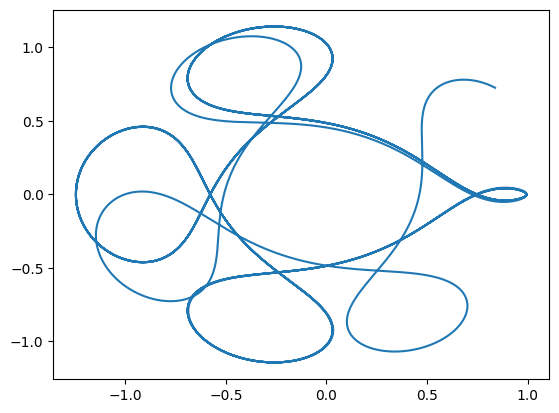
\includegraphics[width = 5cm, height = 4cm]{31.png}
		\caption{Fehlberg, $n=500000$}
		\label{31}
	\end{minipage}
	\qquad
	\begin{minipage}{5cm}
		\centering
		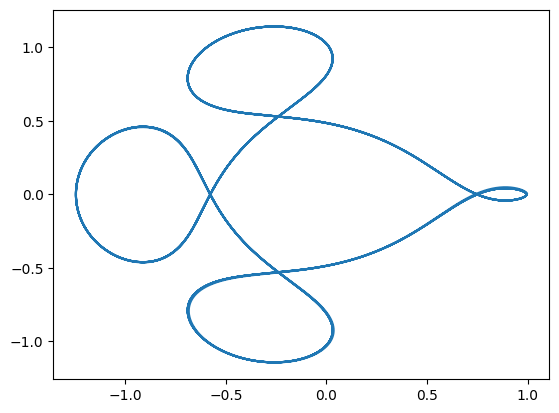
\includegraphics[width = 5cm, height = 4cm]{32.png}
		\caption{Dormand-Prince, $n=500000$}
		\label{32}
	\end{minipage}
\end{figure}

Fehlberg 方法直到第四个周期才略有偏移,第五个周期完全偏移;而 Dormand-Prince 方法直到第五个周期仍非常稳定。另外注意,它们的步数分别只有 $28799$ 和 $26901$。这些任何一种定长单步法都无法做到的。

\section{使用对象工厂进行方法的维护和测试}

本项目使用了对象工厂维护各方法。它可以很方便地将各方法与其名称建立一一对应的联系,且方便添加或删除方法。

\begin{lstlisting}[language=c++]
//IVPSolverFactory.h
#include <bits/stdc++.h>
#include "IVPSolver.h"
using namespace std;
class IVPSolverFactory {
public:
	using CreateCallback = unique_ptr<IVPSolver>(*)();
private:
	using CallbackMap = map<string, CreateCallback>;
public:
	static IVPSolverFactory& CreateFactory() {
		static IVPSolverFactory object;
		return object;
	}
	bool Register(string ID, CreateCallback createFn) {
		return callbacks.insert({ID, createFn}).second;
	}
	bool UnRegister(string ID) {
		return callbacks.erase(ID) == 1;
	}
	unique_ptr<IVPSolver> create(string ID) {
		auto it = callbacks.find(ID);
		if(it == callbacks.end()) {
			throw runtime_error("Unknown IVPSolver ID. ");
		}
		return (it->second)();
	}
	private:
		IVPSolverFactory() = default;
		IVPSolverFactory(const IVPSolverFactory &) = default;
		IVPSolverFactory & operator = (const IVPSolverFactory &) = default;
		~IVPSolverFactory() = default;
	private:
		CallbackMap callbacks;
};
\end{lstlisting}

测试程序不再需要写冗长的 \verb|if/else if|,只需注册好所有方法即可。

\begin{lstlisting}[language=c++]
#include <bits/stdc++.h>
#include "Matrix.h"
#include "function.h"
#include "LMM.h"
#include "RK.h"
#include "Emb_RK.h"
#include "IVPSolverFactory.h"
using namespace std;

class F : public Function_nd<double>{
private:
	double mu;
public:
	F(double mu):mu(mu){n=6;}
	Colvec<double> operator()(const Colvec<double>& u) const {
		if (u.row() != 6) throw "Error: Wrong Dimension of Vector!";
		return {
			u[3],
			u[4],
			u[5],
			2*u[4]+u[0]
			-mu*(u[0]+mu-1)		/pow(u[1]*u[1]+u[2]*u[2]+(u[0]+mu-1)*(u[0]+mu-1),1.5)
			-(1-mu)*(u[0]+mu)	/pow(u[1]*u[1]+u[2]*u[2]+(u[0]+mu)*(u[0]+mu)	,1.5),
			-2*u[3]+u[1]
			-mu*u[1]			/pow(u[1]*u[1]+u[2]*u[2]+(u[0]+mu-1)*(u[0]+mu-1),1.5)
			-(1-mu)*u[1]		/pow(u[1]*u[1]+u[2]*u[2]+(u[0]+mu)*(u[0]+mu)	,1.5),
			-mu*u[2]			/pow(u[1]*u[1]+u[2]*u[2]+(u[0]+mu-1)*(u[0]+mu-1),1.5)
			-(1-mu)*u[2]		/pow(u[1]*u[1]+u[2]*u[2]+(u[0]+mu)*(u[0]+mu)	,1.5)
		};
	}
};

double T[2] = {17.06521656015796, 19.140540691377};
Colvec<double> u0[2] = {
	{0.994, 0, 0, 0, -2.0015851063790825224, 0},
	{0.879779227778, 0, 0, 0, -0.379677780949, 0}
};

int main(int argc, char** argv) {
	IVPSolverFactory& Factory = IVPSolverFactory::CreateFactory();
	Factory.Register("Adam-Bashforth", []() -> unique_ptr<IVPSolver>{return make_unique<Adam_Bashforth>();});
	Factory.Register("Adam-Moulton", []() -> unique_ptr<IVPSolver>{return make_unique<Adam_Moulton>();});
	Factory.Register("BDF", []() -> unique_ptr<IVPSolver>{return make_unique<BDF>();});
	Factory.Register("Classical-RK", []() -> unique_ptr<IVPSolver>{return make_unique<Classical_4th_RK>();});
	Factory.Register("ESDIRK", []() -> unique_ptr<IVPSolver>{return make_unique<ESDIRK>();});
	Factory.Register("Gauss-Legendre-1", []() -> unique_ptr<IVPSolver>{return make_unique<Gauss>(1);});
	Factory.Register("Gauss-Legendre-2", []() -> unique_ptr<IVPSolver>{return make_unique<Gauss>(2);});
	Factory.Register("Gauss-Legendre-3", []() -> unique_ptr<IVPSolver>{return make_unique<Gauss>(3);});
	Factory.Register("Fehlberg", []() -> unique_ptr<IVPSolver>{return make_unique<Fehlberg_Emb_RK>();});
	Factory.Register("Dormand-Prince", []() -> unique_ptr<IVPSolver>{return make_unique<Dormand_Prince_Emb_RK>();});

	string name = argv[1];
	if (name == "Gauss-Legendre") name = name + '-' + argv[2];
	int s = atoi(argv[2]), n = atoi(argv[3]), type = atoi(argv[4]);

	F f(0.012277471);
	unique_ptr<IVPSolver> Solver = Factory.create(name);
	vector<Colvec<double>> u = Solver->Solve(f, u0[type], T[type], n, s);

	if (argc > 4) {
		ofstream out(argv[6]);
		cout << "x,y";
		for (int i = 0; i <= n; ++ i) out << u[i][0] << ',' << u[i][1] << '\n';
		out.flush();
	}
}
\end{lstlisting}

\subsection{八种方法达到 $10^{-3}$ 误差所需步数对比}

最后,我们给出八种方法一个周期误差的无穷范数达到 $10^{-3}$ 的最小步数和时间。所有方法均取最高阶。

使用二分法。见\verb|main2.cpp|。

\begin{table}\centering
	\begin{tabular}{|c|c|c|}
	\hline
	方法 & 步数 & 时间 \\ \cline{1-3}
	Adam-Bashforth & 406557 & 2146\\ \cline{1-3}
	Adam-Moulton & 978649 & 25916\\ \cline{1-3}
	BDF & 352940 & 6207\\ \cline{1-3}
	Classical-RK & 85645 & 961\\ \cline{1-3}
	ESDIRK & 66138 & 8795\\ \cline{1-3}
	Gauss-Legendre & 17183 & 812\\ \cline{1-3}
	Fehlberg & $\approx 800$ & $\approx 35$\\ \cline{1-3}
	Dormand-Prince & $\approx 800$ & $\approx 35$\\ \cline{1-3}
\end{tabular}
\caption{各种方法误差达到 $10^{-3}$ 的最小步数和最短时间}
\end{table}

注意:动态步长龙格库塔方法的最小步数和时间无法精确计算。因为它不是直接控制步长而是通过控制 $\epsilon$ 控制步长。

可见动态步长龙格库塔方法从达到给定误差的角度上也是比定长龙格库塔方法优秀的。

\end{document}